\documentclass[border=5pt]{standalone}
\usepackage[T1]{fontenc}
\usepackage{lmodern,amsmath}
\usepackage{pgfplots}
\pgfplotsset{compat=1.18}
\begin{document}
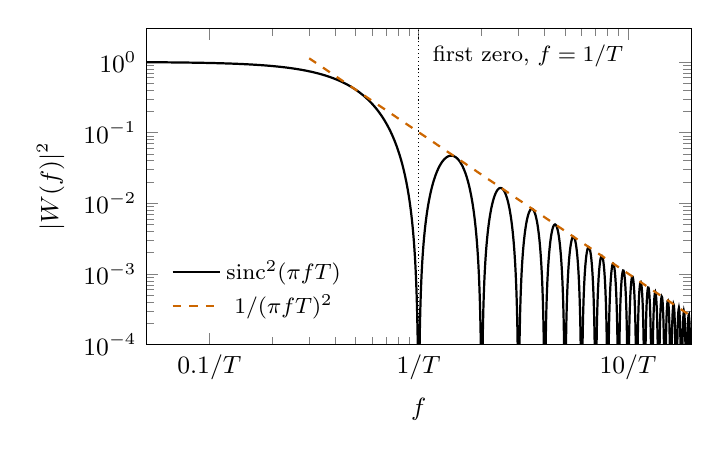
\begin{tikzpicture}[font=\small]
\begin{axis}[width=8.5cm,height=5.6cm,
  xmode=log,ymode=log,xmin=0.05,xmax=20,ymin=1e-4,ymax=3,
  xtick={0.1,1,10},xticklabels={$0.1/T$,$1/T$,$10/T$},
  ytick={1e-4,1e-3,1e-2,1e-1,1},
  xlabel={$f$},ylabel={$|W(f)|^2$},
  legend style={at={(0.03,0.05)},anchor=south west,draw=none,fill=none,font=\footnotesize},
  samples=1200,domain=0.05:20]
\addplot[black,thick,unbounded coords=jump] {max(1e-6,(sin(deg(pi*x))/(pi*x))^2)};
\addlegendentry{$\mathrm{sinc}^2(\pi fT)$}
\addplot[orange!80!black,dashed,thick,domain=0.3:20] {1/(pi*x)^2};
\addlegendentry{$1/(\pi fT)^2$}
\draw[densely dotted] (axis cs:1,1e-4) -- (axis cs:1,3);
\node[anchor=west,font=\footnotesize] at (axis cs:1.05,1.2) {first zero, $f=1/T$};
\end{axis}
\end{tikzpicture}
\end{document}
